\documentclass[conference,spanish]{IEEEtran}

\usepackage{babel}
\usepackage[utf8]{inputenc}
\usepackage[T1]{fontenc}
\usepackage{textcomp}
\usepackage[inline,shortlabels]{enumitem}
\usepackage{amsmath}
\usepackage{caption}
\usepackage{subcaption}
\usepackage{color}
\usepackage{booktabs}
\usepackage{listings}
\usepackage{algorithm}
\usepackage{algpseudocode}
\usepackage[section]{placeins}
\usepackage{pgfplots}
\usepackage[hidelinks]{hyperref}
\usepackage{cleveref}

% Numeros ordenados por entrada
\bibliographystyle{ieeetr} 

% Correcciones para el paquete algorithmic
\floatname{algorithm}{Algoritmo}
\renewcommand{\listalgorithmname}{Lista de algoritmos}
\renewcommand{\algorithmicrequire}{\textbf{Entrada:}}
\renewcommand{\algorithmicensure}{\textbf{Salida:}}
\renewcommand{\algorithmicend}{\textbf{fin}}
\renewcommand{\algorithmicif}{\textbf{si}}
\renewcommand{\algorithmicthen}{\textbf{entonces}}
\renewcommand{\algorithmicelse}{\textbf{si no}}
\renewcommand{\algorithmicfor}{\textbf{para}}
\renewcommand{\algorithmicforall}{\textbf{para todo}}
\renewcommand{\algorithmicdo}{\textbf{hacer}}
\renewcommand{\algorithmicwhile}{\textbf{mientras}}
\renewcommand{\algorithmicloop}{\textbf{repetir}}
\renewcommand{\algorithmicrepeat}{\textbf{repetir}}
\renewcommand{\algorithmicuntil}{\textbf{hasta que}}
\renewcommand{\algorithmicreturn}{\textbf{devolver}} 
\renewcommand{\algorithmicprocedure}{\textbf{procedimiento}}
\renewcommand{\algorithmicfunction}{\textbf{función}}


% Para dibujar los gráficos de líneas
\pgfplotsset{width=10cm,compat=1.9}

% Cambia el nombre de "cuadro" a "tabla" cuando se usa \cref
\crefname{table}{tabla}{tablas}

% Incluimos los graficos en formato pdf_tex
\graphicspath{{apartados/figuras/}}

% Para mostrar la numeración de los listados en itálicas
\setlist[enumerate,1]{font=\itshape}

\begin{document}

    \renewcommand{\lstlistingname}{\textbf{Consulta}}
    \renewcommand\tablename{Tabla}
    \floatname{algorithm}{Algoritmo}
    \floatname{table}{Tabla}
  
	% paper title
	% can use linebreaks \\ within to get better formatting as desired
	\title{Aproximación colaborativa del tránsito vehicular basada en aplicaciones móviles}
	
	% author names and affiliations
	% use a multiple column layout for up to three different
	% affiliations
	\author{
		\IEEEauthorblockN{Alfredo Campuzano}
		\IEEEauthorblockA{Facultad Politécnica\\
			Universidad Nacional de Asunción\\
			San Lorenzo - Paraguay\\
			acampuzano@outlook.com}
		\and
		\IEEEauthorblockN{Rubén López}
		\IEEEauthorblockA{Facultad Politécnica\\
			Universidad Nacional de Asunción\\
			San Lorenzo - Paraguay\\
			rubenlop88@gmail.com}
		\and
		\IEEEauthorblockN{Joaquín Lima}
		\IEEEauthorblockA{Facultad Politécnica\\
			Universidad Nacional de Asunción\\
			San Lorenzo - Paraguay\\
			joaquin.lima@pol.una.py}}

	% make the title area
	\maketitle
	
	\begin{abstract}
El aumento del parque automotor en los países en vías de desarrollo representa un problema debido a que sus ciudades no cuentan con infraestructura vial planificada y tampoco con tecnología instalada para monitorear el estado del tráfico, lo cual impide mejorar el tránsito vehicular y deteriora la calidad de vida de los ciudadanos. Aprovechando el crecimiento en la utilización de teléfonos móviles inteligentes, equipados con sensores GPS, surge la posibilidad de utilizar esta tecnología para obtener información sobre el estado del tráfico de forma económica y eficiente. En este trabajo se presentan los detalles de implementación del sistema denominado \emph{Autotracks}, que permite recolectar y procesar información del tránsito vehicular a través de dispositivos móviles para aproximar el estado del tráfico en tiempo real. Se utiliza un esquema de \emph{Floating Car Data} en combinación con técnicas de detección de actividad para monitorear la ubicación de los vehículos en movimiento. La trayectoria real de los mismos es determinada mediante un proceso de \emph{Map Matching}. Todas las trayectorias son agregadas para aproximar el estado del tráfico en un periodo de tiempo dado. Finalmente, se consigue aproximar el estado del tráfico por calles, información que puede ser utilizada posteriormente para introducir o planificar mejoras, rutear vehículos o encontrar caminos alternativos, entre otros.
	\end{abstract}
	
	\begin{IEEEkeywords}
		Map Matching, Floating Car Data, GIS, Activity Recognition, Traffic State Estimation, Mobile Tracking
	\end{IEEEkeywords}

	% For peerreview papers, this IEEEtran command inserts a page break and
	% creates the second title. It will be ignored for other modes.
	\IEEEpeerreviewmaketitle
	
	\section{Introducción}

La congestión del tránsito es uno de los problemas más serios que enfrentan la mayoría de las zonas urbanas hoy en día, el constante aumento del parque de automóviles, el alto uso de vehículos privados y la falta de planificación de las ciudades son algunos de los factores que afectan negativamente la calidad de vida de los ciudadanos. Además, los países en vías de desarrollado carecen de sistemas de control de tránsito debido al alto costo de inversión requerido y en algunos casos tampoco existen servicios proveídos por empresas privadas para este fin. Esta situación dificulta la utilización eficiente de las vías de tránsito existentes, es por eso que se hace evidente la necesidad de recolectar y analizar información sobre el tránsito de forma barata y sencilla. Los sistemas de información de tráfico basados en \emph{Floating Car Data} (FCD) han demostrado ser una alternativa viable para obtener esta información de forma económica y eficiente \cite{schafer2002traffic,reinthaler2007evaluation}.

Los sistemas existentes de FCD se basan en la utilización de vehículos sonda equipados con sensores GPS. Para este propósito se han utilizado flotas de taxis \cite{schafer2002traffic,reinthaler2007evaluation} y sistemas instalados por empresas de seguro en los vehículos de sus clientes \cite{giovannini2011novel}. Sin embargo, en países menos desarrollados no existen programas o iniciativas públicas y/o privadas que promuevan la utilización de este tipo de sistemas.

Otra alternativa para recolectar FCD es la utilización de teléfonos móviles inteligentes, equipados con sensores GPS, ya que los automovilistas generalmente llevan consigo este tipo de teléfonos. Este tipo de tecnología ya se ha utilizado en aplicaciones para el rastreo de vehículos \cite{thiagarajan2010cooperative}, estimación del tiempo de llegada de buses \cite{zhou2012long} y estimación de tiempo de viaje \cite{thiagarajan2009vtrack}. Diversos estudios han demostrado la factibilidad de utilizar esta tecnología para estimar el estado del tráfico en tiempo real \cite{tao2012real,herrera2010evaluation}, sugiriendo que una penetración de entre un 2 y 3\% es suficiente para proporcionar mediciones precisas de la velocidad del flujo del tráfico \cite{herrera2010evaluation}.

Para estimar el estado del tráfico primeramente se debe determinar la trayectoria de los vehículos por las calles de la ciudad, este proceso es conocido por el nombre de \emph{Map Matching} (MM). Existe una gran variedad algoritmos de MM, desde los más sencillos, basados solamente en información geográfica \cite{white2000some}, hasta los más complejos, basados en modelos estadísticos y otras técnicas avanzadas \cite{quddus2006high,kim2001adaptive}. Debido a las limitaciones impuestas por las plataformas móviles, tales como restricciones de consumo de batería, conectividad limitada o intermitente, errores de precisión, entre otros, resulta necesaria la utilización de algoritmos de MM especializados en procesar muestras relativamente dispersas y poco precisas \cite{lou2009map}.

En este trabajo se describe la implementación de un sistema que permite aproximar las condiciones del tránsito utilizando información proveída por dispositivos móviles en tiempo real. La solución propuesta está basada en FCD obtenido mediante una aplicación móvil desarrollada para el efecto, denominada \emph{Autotracks}, que se instala en los dispositivos de los usuarios y envía periódicamente la información obtenida a un servidor central. Para minimizar el impacto en el consumo de batería, se utiliza un mecanismo de reconocimiento de actividad que permite rastrear al usuario sólo cuando se encuentra en un vehículo en movimiento. Las trayectorias recolectadas son procesadas en el servidor utilizando un algoritmo de MM. La información resultante es almacenada en una base de datos GIS y luego es agregada para obtener una aproximación del estado del tráfico.

El resto del trabajo está organizado de la siguiente forma:
\begin{itemize}
\item El \Cref{sec:recoleccion_datos} describe las técnicas de recolección de información de tráfico. 
\item En el \Cref{sec:map_matching} se describe el problema de MM y los distintos tipos de algoritmos existentes en la actualidad. 
\item En el \Cref{sec:medidas_trafico} se explican los diferentes parámetros que caracterizan el flujo de tráfico. 
\item En el \Cref{sec:arquitectura} se presenta la solución propuesta, su arquitectura, las técnicas seleccionadas para la recolección y el análisis de datos, y los algoritmos utilizados en cada paso del proceso. 
\item En el \Cref{sec:pruebas} se describen las pruebas realizadas y se realiza un análisis de los resultados para verificar el funcionamiento del sistema. 
\item Finalmente, en el \Cref{sec:conclusiones} se exponen las conclusiones finales y trabajos futuros.
\end{itemize}

	\section{Recolección de datos de tráfico}
\label{sec:recoleccion_datos}

Actualmente existen una variedad de tecnologías para la recolección automática de datos del tráfico. Se pueden dividir estas tecnologías en dos categorías. La primera es la \emph{tecnología in-situ}, que toma los datos del tráfico a través de detectores ubicados a lo largo del camino y que vuelve a dividirse en dos categorías: la \emph{intrusiva} y la \emph{no intrusiva}. La segunda, denominada \emph{Floating Car Data} (FCD), obtiene datos del tráfico mediante el uso de vehículos sonda equipados con dispositivos de medición \cite{mimbela2003summary}.

Las \emph{tecnologías de detección in-situ} se basan en la recolección de datos mediante dispositivos específicos para este fin, que son dispuestos físicamente en los lugares sujetos de medición. Se dividen en dos categorías: \begin{enumerate*}[a)] \item las tecnologías \emph{intrusivas}, que están montadas en o por debajo de la superficie de las rutas y cuya instalación ocasiona la interrupción potencial del tráfico (ej: tubos neumáticos y magnetómetros) y \item las tecnologías \emph{no intrusivas}, que son montadas encima o sobre la superficie de las rutas y cuya instalación no genera interrupción del tráfico, o lo hace en pequeña medida (ej: cámaras fotográficas o de video).\end{enumerate*}

Además de la utilización de tecnologías in-situ, muchas aplicaciones de gestión de tráfico utilizan dispositivos montados en vehículos en circulación, conocidos como sistemas de ubicación automática de vehículo (\emph{Automatic Vehicle Location} - AVL). Los dispositivos AVL pueden proveer dos tipos de información: \begin{enumerate*}[a)]
\item información de posición, cuando un vehículo equipado con ellos pasa cierto punto de la red donde existe un sensor, o \item información continua, a medida que el vehículo transita a través de la red.
\end{enumerate*}
Los vehículos sonda pueden ser equipados con dispositivos AVL dedicados o se pueden utilizar dispositivos móviles, tales como teléfonos celulares, que actúan como dispositivos AVL cuando su usuario viaja en vehículo.  

Un sistema basado en FCD consiste en recolectar y procesar datos de tráfico obtenidos en tiempo real, a través de dispositivos AVL montados en vehícuos que circulan en una red de caminos sujeta a observación. Todos los vehículos equipados con estos dispositivos actúan como sensores dentro de la red de caminos. Datos como la ubicación del vehículo, la velocidad y dirección del viaje son recabados para su procesamiento. Luego de la recolección y extracción de los datos, informaciones útiles tales como el estado del tráfico y rutas alternativas, pueden ser derivadas y posteriormente distribuidas.


	\section{Map Matching}
\label{sec:map_matching}

Se conoce como \emph{Map Matching} (MM) al proceso de identificar la trayectoria seguida por un vehículo en una red de calles a partir de muestras dispersas y poco precisas. Este proceso es utilizado en una gran variedad de servicios y aplicaciones de información geográfica, como la predicción de trayectorias de usuarios \cite{eisner2011algorithms}, sistemas de navegación en vehículos \cite{kim2001adaptive}, control del estado del tránsito \cite{thiagarajan2009vtrack}, estimación de llegada de buses \cite{thiagarajan2010cooperative}, entre otros.

Para la realización de un proceso de MM deben tenerse en cuenta los siguientes conceptos:

\textbf{Muestra o Punto}: Una muestra o punto $p$ es el conjunto de todas las mediciones recolectadas por el vehículo en un instante dado. Estas mediciones incluyen la localización del vehículo, su dirección de desplazamiento, su velocidad, etc.

\textbf{Trayectoria}: Una trayectoria $T$ es una secuencia ordenada de muestras o puntos pertenecientes a un vehículo sujeto de observación, recolectados durante un viaje del mismo.

\textbf{Red de calles}: Una red de calles $G(V,E)$ consiste en un grafo dirigido que representa la forma y las propiedades del sistema de calles de un área geográfica en particular. Los vértices $v \in V$ describen las intersecciones entre las calles y las aristas $e \in E$ representan la forma y los atributos de las calles.

\textbf{Camino reconstruido}: Un camino reconstruido $R$ es una secuencia ordenada de calles $e$  conectadas entre sí, a través de las cuáles se infiere que el vehículo pudo haber transitado.

Así, el problema de MM puede definirse de la siguiente forma: \emph{Dada una trayectoria $T$ y una red de calles $G(V,E)$, encontrar el camino $R$ que hace coincidir a $T$ con su reconstrucción más realista sobre $G(V,E)$.}

\subsection{Clasificación de algoritmos de MM}

De acuerdo a la información y las técnicas utilizadas para su implementación los algoritmos de MM se pueden clasificar en: \begin{enumerate*}[1)]\item \emph{geométricos}, que utilizan sólo la información de posición y distancia entre las calles y puntos \cite{white2000some}, son sencillos de implementar y suelen utilizarse como paso inicial en la implementación de otros algoritmos; \item \emph{topológicos}, que incorporan información topológica de la red de calles \cite{lou2009map,yuan2010interactive,greenfeld2002matching,quddus2003general}, utilizan información sobre la conectividad, restricciones de giro, sentido y límite de velocidad de las calles; \item \emph{estadísticos}, que definen regiones de probabilidad alrededor de cada punto y analizan los tramos dentro de dichas regiones \cite{ochieng2009map}, estos análisis estadísticos también se utilizan como parte de otros algoritmos, y \item \emph{avanzados}, que combinan diversas técnicas geométricas, topológicas y estadísticas con otros conceptos tales como \emph{Filtros de Kalman}, \emph{Modelos Ocultos de Markov}, \emph{Lógica Difusa}, entre otros \cite{thiagarajan2009vtrack,quddus2006high,thiagarajan2011accurate,fang2011enacq}\end{enumerate*}.

De acuerdo al momento en el que se realiza el procesamiento de los datos, existen dos categorías: \begin{enumerate*}[1)] \item los algoritmos \emph{incrementales} u \emph{on-line}, que realizan el proceso de MM a medida que se van obteniendo nuevos puntos \cite{thiagarajan2009vtrack,thiagarajan2011accurate,greenfeld2002matching,quddus2003general,quddus2006high} y se utilizan en aplicaciones de tiempo real como asistentes personales de navegación, y \item los algoritmos \emph{globales} u \emph{off-line}, que realizan el proceso MM luego de que se han recolectado todos los puntos \cite{lou2009map,yuan2010interactive} y se utilizan en aplicaciones de análisis de tráfico o estudios sobre el comportamiento de usuarios\end{enumerate*}.

Dependiendo de la frecuencia de muestreo se pueden identificar dos categorías más: \begin{enumerate*}[1)] \item los algoritmos para \emph{alta frecuencia} o \emph{high-sampling}, que típicamente trabajan con intervalos de muestra en el rango de los pocos segundos y generalmente se ejecutan de forma \emph{on-line} \cite{greenfeld2002matching,quddus2003general,quddus2006high}, y \item los algoritmos para \emph{baja frecuencia} o \emph{low-sampling},  que funcionan para intervalos de muestreo de varios minutos y se ejecutan generalmente de forma \emph{off-line} \cite{lou2009map,yuan2010interactive}. \end{enumerate*} En general todos los algoritmos pueden ser alimentados con muestras de alta o baja frecuencia, pero ciertos algoritmos dejan de ser efectivos a medida que disminuye la frecuencia de muestreo.
	\section{Medidas de tráfico}
\label{sec:medidas_trafico}

El tráfico vehicular, o simplemente tráfico, es el fenómeno causado por el flujo de vehículos en una vía, calle o autopista. Cuando el flujo de tráfico es elevado en una zona particular, se produce la congestión del tráfico que deriva principalmente en pérdida de tiempo y consumo extra de combustible para los conductores \cite{litman2011smart}. Las medidas del flujo de tráfico proporcionan información acerca de su naturaleza, lo cual ayuda al análisis de las características del flujo.

Las medidas se pueden clasificar principalmente en: \begin{enumerate*}[a)]
\item mediciones de cantidad, que incluyen la densidad y el volumen de tráfico; y \item mediciones de calidad, que incluye la velocidad
\end{enumerate*}. Las medidas del flujo de tráfico pueden ser: \begin{enumerate*}[a)] \item macroscópicas, que caracterizan el tráfico como un todo; o \item microscópicas, que estudian el comportamiento de vehículos individuales \end{enumerate*}. Las medidas principales para un flujo de tráfico son: \emph{velocidad}, \emph{volumen}, y \emph{densidad} \cite{may1990fundamentals}

La \emph{Velocidad} está definida por el desplazamiento por unidad de tiempo. La velocidad observada por lo general varía de un vehículo a otro. Para representar esa variación, varios tipos de velocidad pueden ser definidos \cite{may1990fundamentals}. Los más importantes entre ellos son: 
\begin{enumerate}

\item La \emph{velocidad de circulación}, que se refiere a la velocidad promedio observada para un recorrido siempre que el vehículo se encuentre en movimiento, no considerándose los intervalos de tiempo en el que el vehículo se encuentre detenido.

\item La \emph{velocidad de viaje}, que está dada por la distancia recorrida entre dos puntos, dividida por el total del tiempo utilizado por el vehículo para completar el viaje, incluyendo los tiempos de parada.

\item La \emph{velocidad media local}, definida como el promedio de velocidad de circulación de todos los vehículos que pasan por un punto de la carretera en un periodo de tiempo determinado.

\item La \emph{velocidad media en un tramo}, definida como el promedio de velocidad de viaje de todos los vehículos que transitan una sección de la carretera durante un periodo de tiempo específico.
\end{enumerate}

El \emph{volumen} se define como el número de vehículos que pasan por una carretera, o por un carril o dirección del camino durante un intervalo de tiempo. La medición se lleva a cabo contando el número de vehículos que pasan por un punto en particular durante un tiempo definido.

La \emph{densidad} se define como el número de vehículos ocupando una longitud de la carretera o carril en un instante dado y es generalmente expresada en vehículos por kilómetro.

La medida más relevante para la estimación del tráfico en tiempo real es la velocidad. Esta información generalmente es utilizada para reducir la congestión en los caminos, ayudando a los conductores a tomar decisiones basadas en el estado de los mismos.
	\section{Arquitectura}
\label{sec:arquitectura}

A continuación se presentan los detalles de implementación del sistema propuesto. La solución propuesta está basada en FCD obtenido mediante dispositivos móviles. La información obtenida es procesada en el servidor utilizando un algoritmo de MM y el resultado es almacenado en una base de datos GIS para consultas a través de una aplicación móvil y una página web desarrolladas para el efecto.

En la \Cref{fig:arquitectura} se ilustra la arquitectura modular del sistema desarrollado. La plataforma cuenta con tres componentes principales:
\begin{enumerate*}[1)] \item una base de datos GIS que almacena el mapa de calles y las trayectorias de los vehículos, \item una aplicación móvil que captura los datos del trayecto recorrido por los vehículos y \item una aplicación web que procesa los datos obtenidos y genera información sobre el estado del tránsito.  
\end{enumerate*}

\begin{figure}[h*]
	\centering
	\input{apartados/figuras/arquitectura.pdf_tex}
	\caption{\label{fig:arquitectura} Arquitectura del Sistema}	
\end{figure}

\subsection{Almacenamiento de datos}
\label{base-de-datos}

A modo de generar información sobre el estado del tráfico de un área geográfica en particular, se debe contar con un mapa de calles y con un conjunto de trayectorias obtenidas mediante FCD durante un período de tiempo determinado.

El mapa de calles es obtenido de Open Street Maps\footnote{http://www.openstreetmap.org/} (OSM) y almacenado en una base de datos GIS como un grafo dirigido, donde los vértices corresponden a las intersecciones de las calles y las aristas corresponden a los segmentos de calles, la longitud de la calle determina su peso, que es utilizado para el cálculo del camino más corto.

Por otro lado, para almacenar la información de las trayectorias de los usuarios se definen las siguientes tablas:
\begin{enumerate}
\item \textbf{Localizaciones}: En esta tabla se guardan los datos de ubicación que son recibidos periódicamente de los usuarios de la aplicación móvil. Se almacena la fecha, la latitud, la longitud, la velocidad, la dirección, la precisión, altitud y la ruta a la que pertenece. Las localizaciones representan los puntos de una trayectoria.
\item \textbf{Rutas}: Una ruta es un conjunto de localizaciones que sirven como dato de entrada para el proceso de MM. La ruta representa a la trayectoria recorrida por el usuario durante un viaje.
\end{enumerate}

\subsection{Implementación de FCD}
\label{floating-car-data}

La información de FCD es obtenida por medio de una aplicación móvil desarrollada como parte del presente trabajo que ha sido denominada Autotracks\footnote{https://play.google.com/store/apps/details?id=py.com.fpuna.autotracks}. La misma se encarga de capturar, almacenar y enviar periódicamente a un servidor central las trayectorias de los usuarios, además la aplicación sólo captura las localizaciones mientras los usuarios están en un vehículo en movimiento. Para este propósito, Autotracks cuenta con tres componentes principales: 

\subsubsection{Reconocimiento de actividad}
\label{reconocimiento_actividad}

El reconocimiento de actividad consiste en determinar la acción que está realizando una persona en base a un patrón de movimientos observados mediante los sensores con los que cuentan los dispositivos móviles, como el acelerómetro, el giroscopio y los dispositivos GPS integrados. En Autotracks se utiliza una implementación proveída como parte de Google Play Services\footnote{http://developer.android.com/google/play-services/index.html}, denominada Activity Recognition\footnote{http://developer.android.com/training/location/activity-recognition.html} para determinar cuando un usuario se encuentra en un vehículo en movimiento.

El \Cref{alg:deteccion_actividad} muestra el procedimiento ejecutado periódicamente cada vez que se obtiene un resultado del reconocimiento de actividad. Este procedimiento verifica si la toma de localizaciones está o no iniciada y se encarga de iniciarla o finalizarla de acuerdo a la actividad detectada. El resultado de la detección es almacenado para ser utilizado en la siguiente invocación del procedimiento. Si se ha detectado movimiento, el tiempo en el que ocurrió la detección también es almacenado.
 
\begin{algorithm}
\caption{Reconocimiento de Actividad}
\label{alg:deteccion_actividad}
\begin{algorithmic}[1]
\Procedure{ActividadDetectada}{$actividad$}
	\State $enVehiculo =$ \Call {EstaEnVehiculo}{$actividad$}
%	\State Guardar $enVehiculo$ como el último estado detectado  
	\If {$enVehiculo$}
		\State $ultimoEstado = \text{VEHICULO}$
		\If {RASTREO no está iniciado}
			\State Iniciar RASTREO
		\EndIf
	\Else
		\State $ultimoEstado = null$
		\If {RASTREO está iniciado}
			\State Finalizar RASTREO
		\EndIf
	\EndIf
\EndProcedure
\Statex
\Function {EstaEnVehiculo}{$actividad$}
	\If {$actividad == \text{A\_PIE}$}
		\State \Return $falso$
	\Else
		\State Inicializar $t$ al tiempo actual
		\If {$actividad == \text{VEHICULO}$}
			\State $t\_ultimaDeteccion = t$ 
			\State \Return $verdadero$
		\Else
		\If {$ultimoEstado == \text{VEHICULO}$}
			\State $\Delta t = t - t\_ultimaDeteccion$
			\If {$\Delta t \leq$ TOLERANCIA}
				\State \Return $verdadero$
			\Else
				\State \Return $falso$
			\EndIf
		\Else
			\State \Return $falso$
		\EndIf
		\EndIf
	\EndIf
\EndFunction
\end{algorithmic}
\end{algorithm}

\subsubsection{Toma de localizaciones}
\label{toma_localizaciones}

La ubicación de los teléfonos móviles puede ser obtenida utilizando triangulación de antenas de telefonía, puntos de acceso WiFi con ubicaciones conocidas o mediante el uso de los satélites GPS. A fin de tener la mayor flexibilidad posible, Autotracks es capaz de trabajar con cualquiera de estas opciones, para ello se utiliza una implementación denominada \emph{Fused Location Provider}\footnote{http://developer.android.com/training/location/receive-location-updates.html}.

En los casos en los que la localización es obtenida a través de las redes GSM o WiFi no se dispone de la información de velocidad, la cual es necesaria para el procesamiento posterior. Para paliar esta falta de información, la velocidad es estimada utilizando la localización anterior de la siguiente manera: \begin{equation} \label{eq:velocidad} v=\frac { d }{ t } \end{equation} donde $d$ es la distancia entre la localización actual y la anterior, y $t$ es el tiempo que transcurrió entre la toma de las localizaciones.

Para evitar registrar localizaciones erróneas se utilizan dos métodos de filtrado. El primer método consiste en descartar las localizaciones que reportan una precisión mayor a un máximo preestablecido. El segundo método consiste en determinar la velocidad de viaje entre dos puntos consecutivos utilizando la \cref{eq:velocidad}, si es mayor a un valor preestablecido la localización es descartada. Además, también se descartan las localizaciones que son muy próximas entre sí. En el \Cref{alg:toma_de_localizaciones} se describe el procedimiento utilizado para registrar una localización.

\begin{algorithm}
\caption{Toma de Localizaciones}
\label{alg:toma_de_localizaciones}
\begin{algorithmic}[1]
\Procedure {Registrar}{$localizacion$}
	\State $esValida = \Call{EsValida}{localizacion}$
	\If {$esValida$}
		\State $ultimaLocalizacion = localizacion$
	\EndIf
\EndProcedure
\Statex
\Function {EsValida}{$localizacion$}
	\State Inicializar $p$ a la precisión de la $localizacion$	
	\State $\Delta d = \Call{Distancia}{localizacion, ultimaLocalizacion}$
	\State $\Delta t = \Call{Tiempo}{localizacion, ultimaLocalizacion}$
	\State $v = \Delta d / \Delta t$
	\If {$\Delta d > \text{D\_MIN} \land v < \text{V\_MAX} \land p < \text{P\_MAX}$}
	    \State \Return $verdadero$
	\Else
	    \State \Return $falso$
	\EndIf
\EndFunction
\end{algorithmic}
\end{algorithm}

\subsubsection{Envío de datos}

La aplicación envía los datos de las localizaciones a través de Internet a un servidor central que se encarga de almacenar y procesar la información. Para disminuir el consumo de batería ocasionado por la utilización de la red de datos móviles, los teléfonos almacenan temporalmente las localizaciones capturadas y las envían periódicamente al servidor. Luego de que un grupo de localizaciones ha sido enviado es borrado de la memoria del teléfono.

Para enviar las localizaciones no es necesario que el usuario haya finalizado completamente su recorrido, todas las localizaciones capturadas durante un periodo de tiempo definido son enviadas al servidor. El resto de las localizaciones del mismo recorrido son enviadas en los siguientes periodos. De esta forma los recorridos parciales pueden ser utilizados para estimar el estado del tráfico aproximadamente en tiempo real.

\subsection{Implementación de MM}
\label{implementacion_mm}

Un proceso de Map Matching (MM) es ejecutado cada vez que las trayectorias de los vehículos son enviadas desde los teléfonos móviles al servidor central para determinar el camino real recorrido por cada vehículo. Para realizar este proceso se utiliza el algoritmo propuesto por \cite{lou2009map}, conocido como ST-Matching, con las mejoras propuestas por \cite{budigm2012algorithm} y \cite{sakic2012map}. 

ST-Matching es un algoritmo topológico específicamente diseñado para funcionar de forma \emph{off-line} y con intervalos de tiempo relativamente largos entre las muestras. Su implementación es sencilla comparada con otras técnicas avanzadas como \cite{quddus2006high, newson2009hidden} y no requiere de procesamientos y cálculos matemáticos complejos. Estas características se adecuan a los requerimientos impuestos por la arquitectura de la solución propuesta. 

El algoritmo ST-Matching consta de tres partes principales: \begin{enumerate*}[a)]
\item la \emph{Selección de Candidatos},
\item el \emph{Análisis Espacial y Temporal} y
\item la \emph{Obtención del Resultado}.
\end{enumerate*}

Los datos de entrada del algoritmo de MM son la red de calles, que se describió en el \cref{base-de-datos}, y la trayectoria de un vehículo, obtenida mediante el uso de la aplicación móvil, como se explica en el \cref{floating-car-data}. El resultado de este procesamiento es una aproximación del camino real recorrido por el vehículo.

La red de calles es modelada como un grafo dirigido $G(V,E)$, donde $V$ es el conjunto de todos los vértices correspondientes a las intersecciones y extremos de los segmentos de calles, y $E$ es el conjunto de todas las aristas que representan segmentos de calles. Además, cada segmento $e \in E$ tiene como datos un identificador único $e.id$, el límite de velocidad $e.v$ de la calle, la longitud $e.l$ del segmento, el identificador del vértice inicial $e.ini$ y el del vértice final $e.fin$. En la \Cref{fig:segmentos_de_calle} se aprecia como una calle puede estar dividida en varios segmentos, donde cada segmento está comprendido entre dos vértices del mapa.

\begin{figure}[h*]
	\centering
	\input{apartados/figuras/segmentos_calle.pdf_tex}
	\caption{\label{fig:segmentos_de_calle} Representación de segmentos de calles}	
\end{figure}

La trayectoria $T$ de un vehículo es representada como una secuencia ordenada de puntos $p_1, p_2, \dots, p_n$ donde cada punto $p_i$ tiene además como datos su latitud $p.lat$, su longitud $p.lon$, su velocidad aproximada $p.v$, su dirección de desplazamiento $p.d$ y el tiempo $p.t$ en que fue tomada la muestra. La trayectoria está ordenada con respecto al tiempo de tal manera que $p_i.t < p_{i + 1}.t$ para $1 \le i < n$. La \Cref{fig:trayectoria} muestra un ejemplo de una trayectoria correspondiente a un vehículo de prueba.

\begin{figure}[h*]
	\centering
	\input{apartados/figuras/trayectoria_vehiculo.pdf_tex}
	\caption{\label{fig:trayectoria} Trayectoria de un vehículo}	
\end{figure}

El camino real $R$ es definido como una secuencia de segmentos de calles $e_i$ conectados entre sí, que se inicia en un vértice $v_{ini} \in V$ y finaliza en un vértice $v_{fin} \in V$, es decir, $R = \{ e_1, e_2, \dots, e_n \}$, donde $e_1.ini = v_{ini}$, $e_n.fin = v_{fin}$ y $e_i.fin = e_{i + 1}.ini$ para $1 \le i < n$.

\subsubsection{Selección de Candidatos}
\label{seleccion_de_candidatos}

La primera etapa del proceso es la selección de puntos candidatos. Un punto candidato $c$ es un punto perteneciente a un segmento de calle $e$, que puede formar parte del camino real recorrido por un vehículo, y que es obtenido a partir de un punto $p$ de una trayectoria. Dada una trayectoria $T = \{p_1, p_2, \dots, p_n\}$, el proceso de selección de candidatos consiste en encontrar para cada punto $p_i$, $1\le i\le n$, el conjunto de puntos candidatos $C_i = \{c_{i}^{1}, c_{i}^{2}, \dots, c_{i}^{m}\}$ correspondiente.

El primer paso es seleccionar todos los segmentos de calles $e \in E$ tales que la distancia entre un punto $p_i$ y un segmento $e$ sea menor a un radio $r$, de esta forma se obtiene un conjunto de segmentos $E_i = \{ e : \text{ } e \in E \text{ } \wedge \text{ } dist(p_i, e) < r \}$. Luego, para cada segmento $e_{i}^{j}$ perteneciente al conjunto $E_i = \{e_{i}^{1}, e_{i}^{2}, \dots, e_{i}^{m}\}$ resultante, se obtiene un punto candidato $c_{i}^{j}$ realizando una proyección del punto $p_i$ sobre el segmento $e_{i}^{j}$. La proyección $proy(p, e)$ de un punto $p$ sobre un segmento $e$ se define como el punto $c$ perteneciente a $e$ más cercano a $p$, es decir, $c = \text{arg } min(dist(c_i, p)) \text{ } \forall c_i \in e$. Así, se obtiene el conjunto de puntos candidatos $C_i = \{ proy(p_i, e_j) \text{ } \forall e_j \in E_i \}$. Como se puede apreciar en la \Cref{fig:puntos_candidatos} un punto candidato puede ser cualquier punto del segmento, como en el caso de $c_{i}^{1}$ y $c_{i}^{2}$, o uno de sus vértices como en el caso de $c_{i}^{3}$.

\begin{figure}[h*]
	\centering
	\input{apartados/figuras/puntos_candidatos.pdf_tex}
	\caption{\label{fig:puntos_candidatos} Puntos candidatos para un punto de la trayectoria}	
\end{figure}

Una vez que se han obtenidos todos los conjuntos $C_i = \{c_{i}^{1}, c_{i}^{2}, \dots, c_{i}^{m}\}$ correspondientes a cada punto $p_i$ de la trayectoria $T$, el problema de MM se reduce a cómo seleccionar un punto candidato $c_i$ de cada conjunto $C_i$, a partir del cual se obtiene el segmento de calle $e_i$, de manera tal que el camino real resultante $R = \{ e_1, e_2, \dots, e_n \}$ sea lo más aproximado posible a $T = \{ p_1, p_2, \dots, p_n\}$.

\subsubsection{Análisis Espacial y Temporal}

La segunda etapa del proceso tiene por objetivo seleccionar el punto candidato $c_i$ de cada conjunto $C_i$ que sea el más apropiado para cada punto $p_i$ de la trayectoria. Para ello cada punto candidato y cada posible conexión entre dos puntos candidatos consecutivos son analizados de acuerdo a dos criterios de calidad, el \emph{análisis espacial} y el \emph{análisis temporal}.

En el análisis espacial se utiliza información geométrica y topológica de la red de calles para evaluar los puntos candidatos. La información geométrica es incorporada utilizando la \emph{probabilidad de observación} y la información topológica es expresada utilizando la \emph{probabilidad de transmisión}.

La \emph{probabilidad de observación} es la probabilidad de que un punto candidato $c_{i}^{j}$ corresponda a un punto $p_i$ de la trayectoria, calculada en base a la distancia $dist(c_{i}^{j},p_i)$ entre los puntos. Asumiendo que el error en la medición de la posición de $p_i$ sigue una distribución normal, la probabilidad de observación $N(c_{i}^{j})$ se define como
\begin{equation} \label{probabilidad_de_observacion}
N(c_{i}^{j}) = \frac {1}{\sqrt { 2 \pi \sigma }} {e}^{\frac {{(x_{i}^{j} - \mu)}^{2}}{{ 2 \sigma}^{2}}}
\end{equation}
donde $x_{i}^{j} = dist(c_{i}^{j},p_i)$ es la distancia entre $p_i$ y el punto candidato $c_{i}^{j}$. 
La \emph{probabilidad de transmisión} se define como la probabilidad de que el camino más corto entre un punto candidato $c_{i-1}^{j}$ y el siguiente punto candidato $c_{i}^{k}$ es el camino correcto de $p_{i-1}$ a $p_i$. La probabilidad de transmisión se calcula de la siguiente forma: 
\begin{equation} \label{probabilidad_de_transmision}
V(c_{i-1}^{j}, c_{i}^{k}) = \frac { min( dist(p_{i-1}, p_i), long(c_{i-1}^{j}, c_{i}^{k})) }{ max (dist(p_{i-1}, p_i), long(c_{i-1}^{j}, c_{i}^{k})) }
\end{equation}
donde $long(c_{i-1}^{j}, c_{i}^{k})$ es la longitud del camino más corto entre $c_{i-1}^{j}$ y $c_{i}^{k}$. El cálculo del camino más corto se realiza utilizando el algoritmo de Dijkstra\footnote{http://es.wikipedia.org/wiki/Algoritmo\_de\_Dijkstra} para grafos dirigidos. La dirección de las aristas del grafo representan el sentido de circulación de la calle, de esta forma se incorpora información topológica en el análisis espacial.

Combinando la \Cref{probabilidad_de_observacion} y la \Cref{probabilidad_de_transmision} se define la función de análisis espacial $F_s(c_{i-1}^{j},c_{i}^{k})$ como el producto de la probabilidad de observación y la probabilidad de transmisión de la siguiente forma:
\begin{equation} \label{funcion_espacial}
F_s(c_{i-1}^{j},c_{i}^{k}) = N(c_{i}^{k}) \times V(c_{i-1}^{j}, c_{i}^{k}), \quad 2 \le i \le n 
\end{equation}

Como resultado del análisis espacial se asigna un valor numérico a todos los posibles caminos que van de $p_{i-1}$ a $p_i$ obtenido mediante la \Cref{funcion_espacial}.

En el análisis temporal calcula la velocidad promedio entre dos puntos consecutivos $p_{i-1}$ y $p_i$ y se compara con los límites de velocidad promedio de los segmentos de calles comprendidos entre dos puntos candidatos $c_{i-1}^{j}$ y $c_{i}^{k}$ con el fin de seleccionar el segmento cuya velocidad promedio es la más cercana a la velocidad promedio de desplazamiento del vehículo.

Dados dos puntos candidatos $c_{i-1}^{j}$ y $c_{i}^{k}$ correspondientes a dos puntos consecutivos $p_{i-1}$ y $p_i$ respectivamente, el camino más corto entre $c_{i-1}^{j}$ y $c_{i}^{k}$ es una lista de segmentos $[e_1, e_2, \dots, e_n]$. La velocidad promedio de desplazamiento del vehículo en este camino más corto se define como:
\begin{equation}
\overline{v} = \frac { \sum_{m=1}^{n} {e_m.l} }{ \Delta t_{i-1, i} }
\end{equation}
donde $e_m.l$ es la longitud del segmento $e_m$ y $\Delta t_{i-1, i} = p_i.t - p_{i-1}.t$ es el intervalo de tiempo entro dos puntos consecutivos de la trayectoria. Además, cada segmento $e_m$ tiene una velocidad $e_m.v$ correspondiente al límite de velocidad de la calle. La Similaridad Coseno\footnote{http://es.wikipedia.org/wiki/Similitud\_coseno} es utilizada para medir la semejanza entre $\overline{v}$ y los límites de velocidad. De esta forma, la función de análisis temporal queda definida así:
\begin{equation} \label{funcion_temporal}
F_{ t }(c_{ i-1 }^{ j },c_{ i }^{ k })=\frac { \sum _{ m=1 }^{ n }{ (e_{ m }.v\times \overline { v } ) }  }{ \sqrt { \sum _{ m=1 }^{ n }{ (e_{ m }.v)^{ 2 } }  } \times \sqrt { \sum _{ m=1 }^{ n }{ (\overline { v } )^{ 2 } }  }  } 
\end{equation}

\subsubsection{Búsqueda del Resultado}

\label{busqueda_de_resultado}
El resultado de los procesos descritos anteriormente es un grafo acíclico dirigido de puntos candidatos, que representa todos los posibles caminos entre el punto inicial $p_1$ y el punto final $p_n$ de la trayectoria $T$. Como se muestra en la \Cref{fig:grafo_de_candidatos}, los nodos del grafo corresponden a los candidatos de cada punto $p_i$ y las aristas representan los caminos más cortos entre cada par de candidatos $c_{i-1}^j$ y $c_i^k$ consecutivos. A cada arista se le asigna un peso de acuerdo a la probabilidad de transmisión entre su vértice inicial y final, y a la probabilidad de observación del vértice inicial.

\begin{figure}[h*]
	\centering
	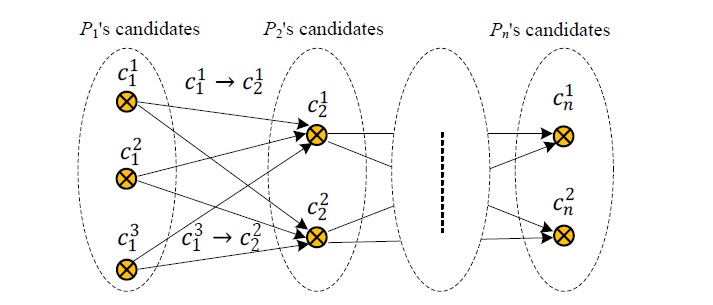
\includegraphics[width=0.45\textwidth]{apartados/figuras/grafo_puntos_candidatos.jpg}
	\caption{\label{fig:grafo_de_candidatos} Grafo de puntos candidatos}	
\end{figure}

Para asignar el peso a cada arista se combinan la \cref{funcion_espacial} y la \cref{funcion_temporal} definiendo así la función espacio-temporal de la siguiente forma:
\begin{equation} \label{funcion_espacio_temporal}
F(c_{i-1}^{j},c_{i}^{k}) = F_s(c_{i-1}^{j},c_{i}^{k}) \times F_{ t }(c_{ i-1 }^{ j },c_{ i }^{ k }), 2 \leq i \leq n
\end{equation}

Dada una secuencia de puntos candidatos $C_T = \{c_1, c_2, \dots, c_n\}$, el peso global se define como $F(C_T) = \sum _{ i=2 }^{ n }{F(c_{i-1}^{j},c_{i}^{k})}$, es decir, es la sumatoria de los pesos de todas las aristas que componen la secuencia. El objetivo del algoritmo es obtener la secuencia que tenga el mayor peso.

El \Cref{alg:st_matching} muestra los pasos realizados para obtener la secuencia de puntos candidatos. El primer paso es construir el grafo $G_T$ de puntos candidatos. Para ello se obtienen todos los conjuntos de puntos candidatos $C_i$ correspondientes a cada punto $p_i$ de la trayectoria $T$. El siguiente paso, es la obtención del resultado final. Primeramente se asigna a todos los candidatos del primer conjunto $C_1$ el valor de su probabilidad de observación $N(c_i^k)$. Luego, para los demás conjuntos $C_i$, se obtienen los valores de la función espacio-temporal para cada par de candidatos consecutivos $c_{i-1}^j$ y $c_i^k$, y para cada $c_i^k$ se guarda el punto candidato previo $c_{i-1}^j$ cuyo valor acumulado sea el mayor. Finalmente se selecciona un punto candidato $c_n^k$ del último conjunto $C_n$, que tenga el valor acumulado más alto y se obtienen todos los puntos candidatos que conforman el camino.

\begin{algorithm}
\caption{ST-Matching}
\label{alg:st_matching}
\begin{algorithmic}[1]
\Procedure {STMatching}{$G:$ grafo de calles, $T:$ trayectoria}
	\State $G_T = \Call{ObtenerCandidatos}{G,T}$
	\State $R = \Call{ObtenerResultado}{G_T}$
	\State \Return $R$
\EndProcedure
\Statex
\Function {ObtenerCandidatos}{$G:$ grafo de calles, $T:$ trayectoria}
	\State Inicializar $G_T$ a un conjunto vacío
	\For {$p_i \in T, 1 \leq i \leq n$} 
		\State $C_i = SeleccionarCandidatos(p_i, G)$
		\State Agregar $C_i$ a $G_T$
	\EndFor
	\State \Return $G_T$
\EndFunction
\Statex
\Function {ObtenerResultado}{$G_T:$ grafo de candidatos}
	\State Definir $f[]$ como el máximo peso computado hasta ahora
	\State Definir $pre[]$ como el padre del punto candidato actual
	\ForAll {$c_1^k$}
		\State $f[c_1^k] = N(c_1^k)$
	\EndFor
	\For {$2 \leq i \leq n$}
		\ForAll {$c_i^k$}
			\State $max = -\infty$
			\ForAll {$c_{i-1}^j$}
				\State $tmp = f[c_{i-1}^j] + F(c_{i-1}^j,c_i^k)$
				\If {$tmp > max$}
					\State $max = tmp$
					\State $pre[c_i^k] = c_{i-1}^j$
				\EndIf
				\State $f[c_i^k] = max$
			\EndFor
		\EndFor
	\EndFor
	\State Inicializar $C$ a una lista vacia de candidados
	\State $c = arg \text{ } max(f[c_n^j])$
	\For {$2 \leq i \leq n$}
		\State Agregar $c$ a $C$
		\State $c = pre[c]$
	\EndFor
	\State Agregar $c$ a $C$
	\State Invertir $C$
	\State \Return $C$
\EndFunction
\end{algorithmic}
\end{algorithm}

\subsection{Estimación del tráfico}
\label{estimacion_trafico}

Una vez finalizado el proceso MM, a cada punto de la trayectoria se le asocia una arista del mapa de calles por la cual se ha determinado que el vehículo transitó en ese momento. Además cada punto de la trayectoria tiene como dato la velocidad a la cual el vehículo se desplazó. Para realizar la estimación del estado del tráfico se utilizan todas las velocidades de los puntos asociados a cada segmento de calle del mapa durante un período de tiempo determinado.

La estimación se realiza calculando la \emph{velocidad media local} de cada segmento de calle. Para ello se define la velocidad media en la calle $j$ durante el intervalo de interés como:
\begin{equation}
\label{eq:velocidad_media}
{ V }_{ ave }^{ j }({ t }_{ k },{ t }_{ k+\Delta T })=\frac { 1 }{ { n }_{ { t }_{ k },{ t }_{ k+\Delta T } }^{ j } } \sum_{ k={ t }_{ k } }^{ { t }_{ k+\Delta T } }{ \hat { { v } } _{ j }(k) }
\end{equation}
donde ${ \hat { { v } } _{ j }(k) }$ es la velocidad estimada en la calle $j$ durante el intervalo $\left[ { t }_{ k },{ t }_{ k+\Delta T } \right] $, y ${ { n }_{ { t }_{ k },{ t }_{ k+\Delta T }}}$ es el número total de muestras disponibles para la calle $j$ durante dicho intervalo.

Finalmente, para representar la información obtenida en intervalos que faciliten su interpretación, se definen cuatro posibles niveles de velocidad en una calle:
\begin{enumerate}
\item \textbf{Rojo:}  para velocidades entre 0 y 14 kilómetros por hora.
\item \textbf{Naranja:}  para velocidades entre 15 y 29 kilómetros por hora.
\item \textbf{Amarillo:}  para velocidades entre 30 y 39 kilómetros por hora.
\item \textbf{Verde:}  para velocidades de 40 o más kilómetros por hora.
\end{enumerate}
Las calles son pintadas en el mapa de acuerdo a su nivel de velocidad como se puede apreciar en la \Cref{fig:calles}.
\begin{figure}[h]
	\centering
	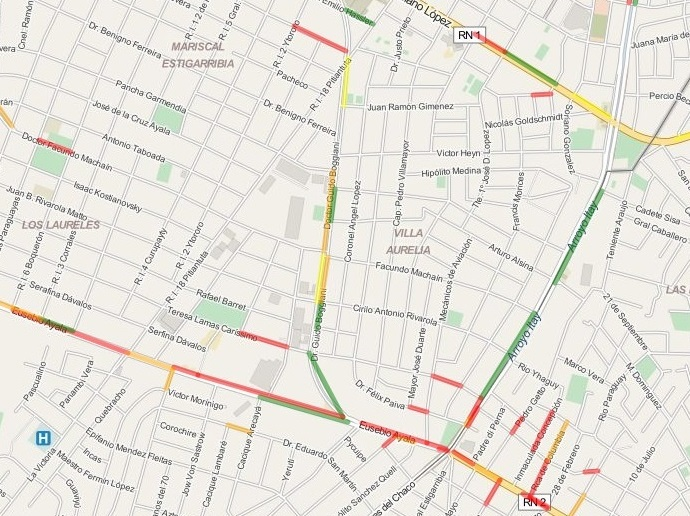
\includegraphics[width=0.45\textwidth]{apartados/figuras/estado_calles.jpg}
	\caption{\label{fig:calles} Estado de calles en Autotracks}	
\end{figure}

	\section{Pruebas y Resultados}
\label{sec:pruebas}

En esta sección se describen las pruebas de campo realizadas y los resultados obtenidos. Un primer grupo de pruebas tuvo por objetivo determinar los valores más adecuados para los parámetros utilizados en la recolección de FCD, tanto en el reconocimiento de actividad como en la toma de localizaciones. Otro grupo de pruebas se realizó con el objetivo determinar la efectividad del sistema implementado, para ello se verificó la tasa de acierto del algoritmo de MM y se analizaron los datos obtenidos para determinar las horas pico y los días con mayor flujo de tráfico.

Debido a la complejidad y a la gran cantidad de variables intervinientes en el funcionamiento del sistema se optó por realizar pruebas de campo en lugar de utilizar simulaciones. Para las pruebas se utilizaron dispositivos móviles de diversa gama y se realizaron tanto en vehículos de transporte público, como en vehículos privados, también se analizaron los datos generados por usuarios reales del sistema. 

\subsection{Deducción de parámetros para FCD}

En la recolección de FCD se utiliza un esquema de detección de actividad que permite a la aplicación registrar las localizaciones del usuario únicamente cuando se encuentra en un vehículo en movimiento. Para ello, la aplicación móvil verifica periódicamente cuál es la actividad que está realizando el usuario en base a las lecturas de los sensores del dispositivo. 

El intervalo de tiempo en el que se realiza la verificación de actividad se denomina \emph{intervalo de reconocimiento} y determina qué tan rápido se detecta el movimiento para iniciar o finalizar el rastreo. Es importante tener en cuenta que mientras más corto es el intervalo, mayor es el consumo de batería debido a que el dispositivo móvil debe procesar más frecuentemente las muestras de los sensores. Para determinar el valor apropiado para el intervalo de reconocimiento se realizaron pruebas empíricas con diferentes valores obteniéndose para cada uno de ellos el tiempo promedio que tarda en detectarse el movimiento. 

La \Cref{tab:prom_intervalo_reconocimiento} muestra el tiempo promedio que la aplicación tarda en detectar el movimiento e iniciar la toma de localizaciones para varios valores del intervalo de reconocimiento. Como se puede apreciar, un intervalo de reconocimiento corto ayuda a iniciar más rápidamente la toma de localizaciones. En base a las pruebas realizadas el intervalo de reconocimiento seleccionado es de 30 segundos, por ser el intervalo más largo que presenta un tiempo de respuesta que no causa pérdidas significativas en el trayecto rastreado.


\begin{table}[h]
  \centering
	\begin{tabular}{ccccc}
	\toprule
	Intervalo (s) & Recorridos & En bus (min.) & En auto (min.) & Ambos (min.) \\
	\midrule
	15            & 30       & 1.55         & 1.25            & 1.40         \\
	30            & 30       & 1.64         & 1.75            & 1.71         \\
	45            & 30       & 2.59         & 2.05            & 2.32         \\
	60            & 30       & 4.37         & 2.75            & 3.66         \\
	\bottomrule
	\end{tabular}
  \caption{Tiempos promedio para inicio de rastreo}
  \label{tab:prom_intervalo_reconocimiento}
\end{table}


El reconocimiento de actividad también es utilizado para detener la toma de localizaciones cuando el usuario ya no se encuentra en un vehículo en movimiento. Se debe tener en cuenta que durante una trayectoria el vehículo puede detenerse momentáneamente debido a diversas causas, como ser un semáforo en rojo o una parada de bus. En estos casos la toma de localizaciones no debe ser erróneamente detenida porque se producirían cortes en la captura del trayecto. 

Para evitar cortes en el rastreo se introduce un \emph{tiempo de tolerancia} en el reconocimiento de actividad para detener el rastreo. Cada vez que se detecta el movimiento, se almacena el tiempo de detección y el rastreo no es detenido hasta que haya transcurrido el tiempo de tolerancia a partir de la última vez que se detectó movimiento. Se debe tener en cuenta también que un tiempo de tolerancia alto implica que se tardará más en detener el servicio de localización, lo que puede producir un impacto negativo en el consumo de batería.

El tiempo que el dispositivo estuvo rastreando al usuario puede ser menor al tiempo total que duró realmente el viaje. El porcentaje de tiempo que el dispositivo estuvo rastreando al usuario con respecto al tiempo total que duró el viaje se denomina \emph{tiempo efectivo de rastreo}. Los valores de tiempo de tolerancia e intervalo de reconocimiento en conjunto influyen en el tiempo efectivo de rastreo por lo que deben ser escogidos apropiadamente.

En la \Cref{tab:prom_tiempo_efectivo_rastreo} se muestra resultados acerca del tiempo efectivo de rastreo observado para diferentes combinaciones de valores de intervalo de reconocimiento y de tiempo de tolerancia considerados. 

\begin{table}[h]
    \centering
	\begin{tabular}{ccccc}
    	\toprule
    	Intervalo (s) & Tolerancia (min.) & En bus (\%) & En auto (\%) & Ambos (\%) \\
    	\midrule
    	15            & 5                 & 89.31         & 93.67          & 91.49        \\
    	30            & 5                 & 85.86         & 91.56          & 88.71        \\
    	45            & 5                 & 83.34         & 89.32          & 86.33        \\
    	60            & 5                 & 80.83         & 87.73          & 84.24        \\
    	15            & 10                & 95.83         & 97.22          & 96.53        \\
    	30            & 10                & 94.44         & 96.11          & 95.28        \\
    	45            & 10                & 89.55         & 95.44          & 92.49        \\
    	60            & 10                & 83.33         & 93.89          & 88.61        \\
    	\bottomrule
	\end{tabular}
    \caption{Tiempos efectivos de rastreo}
    \label{tab:prom_tiempo_efectivo_rastreo}
\end{table}

De las pruebas realizadas puede notarse que con una tolerancia de 10 minutos combinada con un intervalo de reconocimiento de 30 segundos se obtienen coberturas del 95\%, seleccionándose dichos valores como apropiados para este trabajo.

\subsection{Verificación de efectividad de MM}

Para el MM se utiliza el algoritmo ST-Matching como se describe en \cref{implementacion_mm}. Este algoritmo recibe como entrada un conjunto de localizaciones correspondientes a una trayectoria seguida por un usuario, el intervalo de tiempo con el que se obtienen estos puntos se denomina \emph{intervalo de muestreo}. Si el intervalo es grande, se tiene un menor número de muestras para un periodo de tiempo dado y por ende un menor consumo de batería del dispositivo móvil. En cambio, para intervalos pequeños, se tiene un mayor número de muestras y un elevado consumo de batería. Para medir la efectividad del MM, se observa la cantidad de puntos que son correctamente asignados a las calles al estimar el camino real recorrido.

Las pruebas de MM consistieron en la observación de su efectividad con diferentes intervalos de muestreo. Los intervalos observados fueron de 30, 60 y 120 segundos, para cada intervalo se realizaron varios recorridos por un mismo trayecto, se sumó la cantidad total de puntos recolectados y se comparó con la cantidad de puntos correctamente asignados. Los resultados obtenidos pueden ser apreciados en la \Cref{table:map_matching}. Para intervalos pequeños de toma localizaciones se tienen mejores resultados, con una leve diferencia a favor del intervalo de 30 segundos en comparación al intervalo de 60 segundos y con una diferencia un poco mayor en comparación al de 120 segundos. En base a estos resultados se decidió utilizar el intervalo de 60 segundos debido a que consume menos batería y produce resultados similares al intervalo de 30 segundos.

\begin{table}[h]
	\centering
	\begin{tabular}{cccc}
        \toprule
    	Intervalo (s) & Total de Puntos & Puntos Correctos & Tasa de Acierto (\%)\\
    	\midrule
    	30 & 120  & 111 & 93 \\
    	60 & 120 & 109 & 91 \\
    	120 & 120 & 106 & 88 \\ 
    	\bottomrule
	\end{tabular}
	\caption{Efectividad del MM} 
	\label{table:map_matching}
\end{table}

\subsection{Análisis de Tráfico}

Para realizar las pruebas de análisis de tráfico se distribuyó la aplicación Autotracks a través de Google Play\footnote{https://play.google.com/store} y se observaron los resultados obtenidos a durante un periodo de 5 semanas de uso de la aplicación. Durante ese periodo de tiempo un promedio de 212 usuarios utilizaron la aplicación diariamente, generando un total de 123419 puntos observados desde sus dispositivos móviles. Debido a que los usuarios pueden activar o desactivar los sensores de sus teléfonos, no se hace distinción entre los puntos obtenidos a través de GPS, Wifi o triangulación de antenas. En la \Cref{fig:cantidad_usuarios} se observa la cantidad de usuarios activos por día durante el periodo de prueba.

\begin{figure}[h]
	\centering
	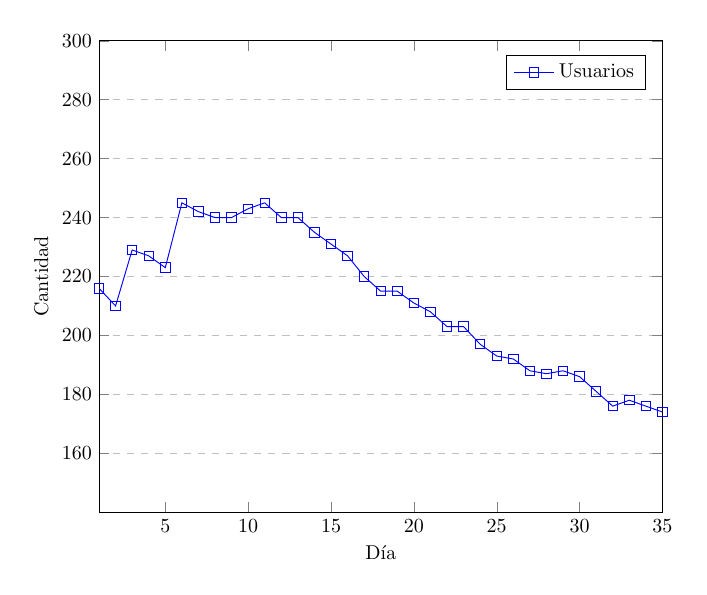
\begin{tikzpicture}[thick,scale=0.85, every node/.style={scale=0.85}]
	\begin{axis}[
	xlabel={Día},
	ylabel={Cantidad},
	xmin=1, xmax=35,
	ymin=140, ymax=300,
	xtick={5,10,15,20,25,30,35},
	ytick={160,180,200,220,240,260,280,300},
	legend pos=north east,
	ymajorgrids=true,
	grid style=dashed,
	]
	
	\addplot[
	color=blue,
	mark=square,
	]
	coordinates {
		(35,174)(34,176)(33,178)(32,176)(31,181)(30,186)(29,188)(28,187)(27,188)(26,192)(25,193)(24,197)(23,203)(22,203)(21,208)(20,211)(19,215)(18,215)(17,220)(16,227)(15,231)(14,235)(13,240)(12,240)(11,245)(10,243)(9,240)(8,240)(7,242)(6,245)(5,223)(4,227)(3,229)(2,210)(1,216)
	};
	\legend{Usuarios}
	
	\end{axis}
	\end{tikzpicture}
	\caption{Cantidad de usuarios activos por día}
	\label{fig:cantidad_usuarios}
\end{figure}

Con el objetivo de caracterizar el flujo de tráfico a lo largo de una semana, se analizó la distribución de la cantidad de puntos recolectados por día de la semana y por hora del día. En la \Cref{table:localizaciones_por_dia} se puede ver la distri
bución por día de la semana, se observa que los lunes son los días en que más localizaciones se reciben, mientras que en los días domingos se recibe el menor número de localizaciones. También se puede apreciar que se recibe una mayor cantidad de localizaciones durante los días entre semana.

\begin{table}[h]
	\centering
	\begin{tabular}{ccc}
        \toprule
    	Día  & Total de Puntos & Promedio\\
    	\midrule
    	Lunes & 20262 & 4052 \\
    	Martes & 18385 & 3677 \\
    	Miércoles & 19361  & 3872 \\ 
    	Jueves & 17833 & 3567 \\
    	Viernes & 18808 & 3762 \\
    	Sábado & 16834 & 3367 \\
    	Domingo & 11936 & 2387 \\
    	\bottomrule
	\end{tabular}
	\caption{Localizaciones tomadas por día de la semana} 
	\label{table:localizaciones_por_dia}
\end{table}

En la \Cref{table:localizaciones_por_hora} se puede observar la distribución de las localizaciones durante las horas del día. Las horas con mayor cantidad de localizaciones recibidas son en la mañana de 6 a 9 y por la tarde de 17 a 19. Durante los días entre semana que son normalmente laborales, se hace más notoria esta diferencia. Mientras que durante los fines de semana la horas con mayor cantidad de localizaciones se encuentran hacia el mediodía.

\begin{table}[!h]
	\centering
	\begin{tabular}{cccc}
        \toprule
    	Hora  & Total & Entre semana & Fin de semana\\
    	\midrule
    	00 & 1947 & 1293 & 654 \\
    	01 & 1061 & 424 & 637 \\
    	02 & 1018 & 414 & 604 \\ 
    	03 & 834 & 368 & 466\\
    	04 & 821 & 424 & 397\\
    	05 & 917 & 621 & 296\\
    	06 & 5236 & 4824 & 412 \\
    	07 & 7931 & 7117 & 814\\
    	08 & 9518 & 8586 & 932\\
    	09 & 7326 & 5900 & 1426\\ 
    	10 & 4710 & 3353 & 1357\\
    	11 & 4904 & 3307 & 1597\\
    	12 & 6727 & 4489 & 2238\\
    	13 & 5636 & 3925 & 1711\\
    	14 & 5190 & 3546 & 1644\\
    	15 & 6128 & 4498 & 1630\\
    	16 & 5868 & 4418 & 1450\\ 
    	17 & 6744 & 5287 & 1457\\
    	18 & 10892 & 9204 & 1688\\
    	19 & 9639 & 8018 & 1621\\
    	20 & 7506 & 5815 & 1691\\
    	21 & 6435 & 4525 & 1910\\
    	22 & 4163 & 2933 & 1230 \\
    	23 & 2214 & 1360 & 854\\
    	\bottomrule
	\end{tabular}
	\caption{Localizaciones tomadas por hora del día} 
	\label{table:localizaciones_por_hora}
\end{table}

Otro parámetro que caracteriza el flujo de tráfico es la velocidad promedio de desplazamiento de los vehículos. En la \Cref{table:velocidad_por_hora} se observa el promedio de velocidad por hora del día. Como se aprecia en la \Cref{fig:promedio_velocidad} por las mañanas el promedio más bajo de velocidad se da entre las 6 y las 9 horas, mientras que por las tardes esto sucede de 18 a 21 horas, también se observa una disminución en la velocidad promedio durante el mediodía. En la \Cref{fig:promedio_velocidad_es_fs} se pueden apreciar las diferencias que existen en los promedios de velocidad de los días entre semana y fines de semana. Durante los días entre semana se observa un promedio menor de velocidad a partir de las 5 horas, esta velocidad promedio se mantiene menor hasta las 19 horas.

\begin{table}[h]
	\centering
	\begin{tabular}{cccc}
        \toprule
    	Hora  & Total(km/h) & Entre semana(km/h) & Fines de semana(km/h)\\
    	\midrule
    	00 & 23.2 & 22.3 & 24.9 \\
    	01 & 27.8 & 24.9 & 29.7 \\
    	02 & 30.8 & 33.1 & 29.2 \\ 
    	03 & 31.9 & 36.8 & 28.1\\
    	04 & 38.2 & 47.3 & 31.2\\
    	05 & 33.3 & 29.9 & 40.4\\
    	06 & 17.7 & 16.8 & 28.5\\
    	07 & 19.5 & 18.9 & 24.8\\
    	08 & 18.1 & 16.9 & 28.8\\
    	09 & 19.5 & 17.6 & 27.4\\ 
    	10 & 24.3 & 19.1 & 24.5\\
    	11 & 21.2 & 20.3 & 22.9\\
    	12 & 19 & 17.8 & 21.4\\
    	13 & 19.2 & 18.5 & 20.7\\
    	14 & 23.6 & 20.9 & 29.4\\
    	15 & 22.1 & 20.1 & 27.7\\
    	16 & 20.8 & 19.4 & 24.9\\ 
    	17 & 20.2 & 18.6 & 26,2\\
    	18 & 16.8 & 15.9 & 21.7\\
    	19 & 17.7 & 16.8 & 22.1\\
    	20 & 18.4 & 18.5 & 18.1\\
    	21 & 18.8 & 18.8 & 18.8\\
    	22 & 21.5 & 22.7 & 18.8\\
    	23 & 21.8 & 22.7 & 20.4\\
    	\bottomrule
	\end{tabular}
	\caption{Promedio de velocidad por hora del día} 
	\label{table:velocidad_por_hora}
\end{table}

\begin{figure}[h]
\centering
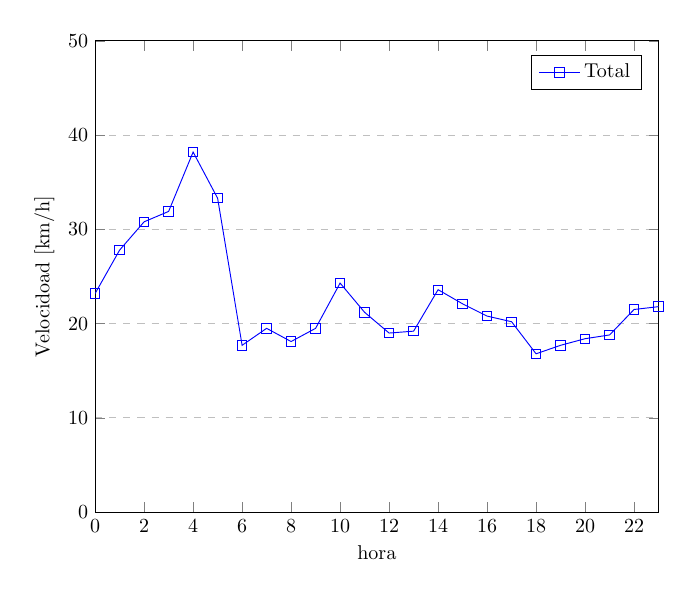
\begin{tikzpicture}[thick,scale=0.85, every node/.style={scale=0.85}]
\begin{axis}[
    xlabel={hora},
    ylabel={Velocidoad [km/h]},
    xmin=0, xmax=23,
    ymin=0, ymax=50,
    xtick={0,2,4,6,8,10,12,14,16,18,20,22},
    ytick={0,10,20,30,40,50},
    legend pos=north east,
    ymajorgrids=true,
    grid style=dashed,
]
 
\addplot[
    color=blue,
    mark=square,
    ]
    coordinates {
    (0,23.2)(1,27.8)(2,30.8)(3,31.9)(4,38.2)(5,33.3)(6,17.7)(7,19.5)(8,18.1)(9,19.5)(10,24.3)(11,21.2)(12,19)(13,19.2)(14,23.6)(15,22.1)(16,20.8)(17,20.2)(18,16.8)(19,17.7)(20,18.4)(21,18.8)(22,21.5)(23,21.8)
    };
    \legend{Total}
 
\end{axis}
\end{tikzpicture}
\caption{Promedio de velocidad por hora del día}
\label{fig:promedio_velocidad}
\end{figure}

\begin{figure}[h]
\centering
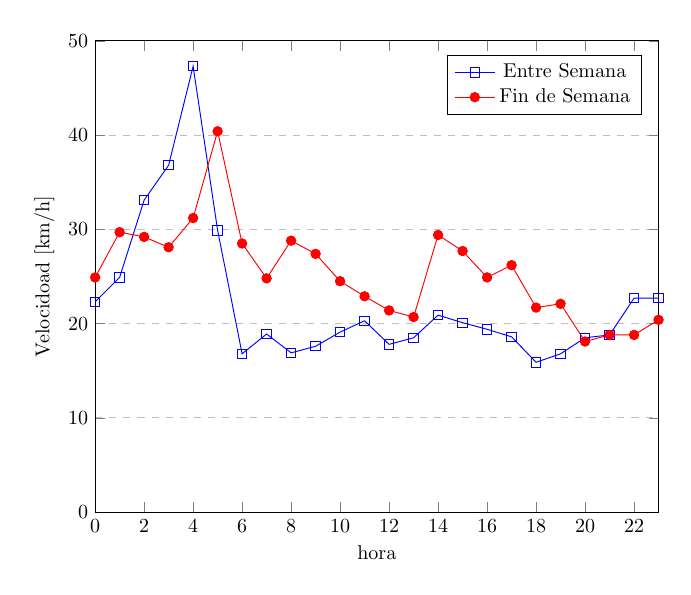
\begin{tikzpicture}[thick,scale=0.85, every node/.style={scale=0.85}]
\begin{axis}[
    xlabel={hora},
    ylabel={Velocidoad [km/h]},
    xmin=0, xmax=23,
    ymin=0, ymax=50,
    xtick={0,2,4,6,8,10,12,14,16,18,20,22},
    ytick={0,10,20,30,40,50},
    legend pos=north east,
    ymajorgrids=true,
    grid style=dashed,
]
 
\addplot[
    color=blue,
    mark=square,
    ]
    coordinates {
    (0,22.3)(1,24.9)(2,33.1)(3,36.8)(4,47.3)(5,29.9)(6,16.8)(7,18.9)(8,16.9)(9,17.6)(10,19.1)(11,20.3)(12,17.8)(13,18.5)(14,20.9)(15,20.1)(16,19.4)(17,18.6)(18,15.9)(19,16.8)(20,18.5)(21,18.8)(22,22.7)(23,22.7)
    };
    \addlegendentry{Entre Semana}

\addplot[
    color=red,
    mark=*,
    ]
    coordinates {
    (0,24.9)(1,29.7)(2,29.2)(3,28.1)(4,31.2)(5,40.4)(6,28.5)(7,24.8)(8,28.8)(9,27.4)(10,24.5)(11,22.9)(12,21.4)(13,20.7)(14,29.4)(15,27.7)(16,24.9)(17,26.2)(18,21.7)(19,22.1)(20,18.1)(21,18.8)(22,18.8)(23,20.4)
    };
    \addlegendentry{Fin de Semana}
 
\end{axis}
\end{tikzpicture}
\caption{Comparativa de Promedio de velocidad por hora del día}
\label{fig:promedio_velocidad_es_fs}
\end{figure}
	\section{Conclusiones}
\label{sec:conclusiones}

En este trabajo se describió la implementación efectiva de un sistema inteligente de información de tráfico, de bajo costo y adecuado a las condiciones de infraestructura de los países en vías de desarrollo. Los datos de FCD son obtenidos mediante dispositivos móviles, utilizando un esquema de reconocimiento de actividad para rastrear los dispositivos únicamente cuando éstos se encuentran dentro de un vehículo en movimiento.

Los datos recolectados durante las pruebas permitieron generar una aproximación del tráfico en la que es posible determinar horas pico y sus velocidades promedio y que además está en concordancia con la realidad percibida diariamente. Se identifica que el mayor volumen de tráfico se da de 6 a 9 de la mañana, al mediodía y entre las 18 y 21 horas, y durante estos periodos se observa una disminución considerable en la velocidad promedio de los vehículos.

También para algunos segmentos de calles en donde se contó con usuarios suficientes y constantes día a día, fue posible proveer en tiempo real información acerca del estado de transito en los mismos.

En base a las pruebas de campo realizadas y los datos recolectados de usuario finales se observa la viabilidad de aplicar dispositivos móviles para aproximar el estado del tránsito cuando no se cuenta con infraestructura instalada para el efecto.

Como trabajos futuros se....
	
	\bibliography{../referencias}

\end{document}	